%!TEX root=thesis.tex
\chapter{Background}

% \section{Motivation}

Some physicists believe that quantum physics is on the cusp of a ``second quantum revolution'' \cite{quantum-rev}. The ability to probe quantum systems with finer precision and control them to a greater extent, as opposed to passively observing emergent phenomena that arise, has the potential to radically transform many different areas, from sensing to simulation to quantum computation.

Hamiltonian engineering is an important problem in the effort to more finely control quantum systems.
Every system has a Hamiltonian that characterizes its dynamics, and as the name suggests, Hamiltonian engineering seeks to ``engineer'' a different Hamiltonian so that the system's dynamics are altered. Hamiltonian engineering has been applied to NMR spectroscopy by engineering Hamiltonians without certain interactions that cause noisier measurements. Engineering Hamiltonians can also be used for sensing (where certain interactions are sensitive to external fields while being robust to decoherence) and for quantum simulation (where novel Hamiltonians must be implemented in existing systems).

Two specific examples where Hamiltonian engineering can be readily applied include NMR spectroscopy and bath engineering. In NMR spectroscopy, the collective magnetization of spin-1/2 protons in a sample can be measured, and the resulting signal informs the particular chemical environments in which the spins exist. However, for solid-state samples, magnetic dipolar interactions between spins lead to state decoherence
and overwhelm the signal, inhibiting our ability to learn about the chemical environments. However, various methods have been developed to effectively \emph{decouple} the magnetic dipolar interactions between spins, improving the signal drastically.

Magnetic dipole interactions between a central spin and many surrounding bath spins (such as an NV center surrounded by many P1 centers) also lead to unwanted effects, in this case a decay of the central spin coherence time. Long coherence times for the system of interest are desirable, and finding ways to decouple interactions between the central spin and bath spins would help that endeavor.

\section{Spin-1/2 Systems and Nuclear Magnetic Resonance}

A spin-1/2 particle (such as an electron or proton) has two possible values for its intrinsic angular momentum or ``spin,'' so the corresponding Hilbert Space for a single spin-1/2 particle has dimension two. $I_x, I_y$ and $I_z$ denote the operators for nuclear spin along $x, y$, and $z$, respectively. When placed in a magnetic field, the magnetic dipole moment (which is proportional to spin) will interact with the field and the spin will begin to precess.
% TODO make a figure showing a single spin and a B field?
For a collection of $N$ spin-1/2 particles, the corresponding Hilbert Space has dimension $2^N$.
For an ensemble of spins, the term $I_z^{(j)}$ is shorthand for a tensor product of operators, all identity except for the $j$th operator
\[
I_z^{(j)} = \identity \otimes \identity \otimes \dots \otimes I_z \otimes \dots \otimes \identity
\]
Similarly, the term $I_z^{(j)}I_z^{(k)}$ is shorthand for a product of identity operators except for the $j$th and $k$th operators.

Nuclear magnetic resonance (NMR) encompasses the study of nuclear spins and the various interactions they have with external fields and with each other.
The key interactions considered in this work are given below in equations~\ref{eq:nmr-ham} through~\ref{eq:nmr-ham-rf}, but a complete description of the interactions present in NMR can be found in \cite{1976ii}.%
\footnote{The quadrupolar interaction and J coupling are not considered here, but it's good to remember they're still there in general.}
Figure~\ref{fig:spin-system} graphically depicts a spin system and the dipolar interactions between spins.

\begin{figure}[H]
    \centering
    

\tikzset{every picture/.style={line width=0.75pt}} %set default line width to 0.75pt        

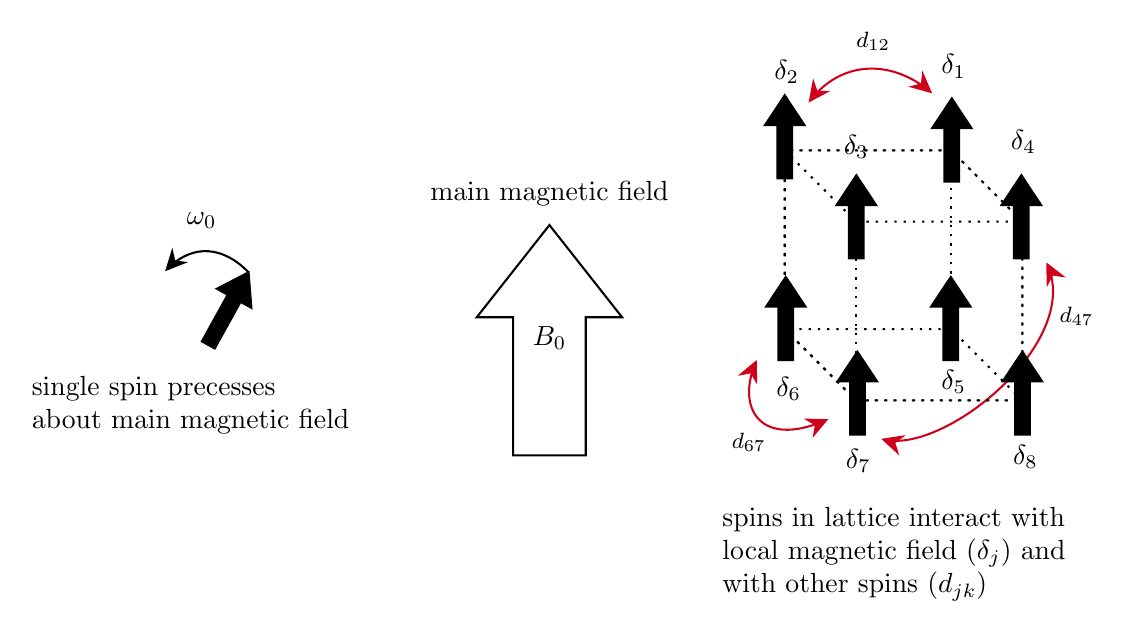
\begin{tikzpicture}[x=0.75pt,y=0.75pt,yscale=-1,xscale=1]
%uncomment if require: \path (0,379); %set diagram left start at 0, and has height of 379

%Up Arrow [id:dp7271723556391365] 
\draw  [fill={rgb, 255:red, 0; green, 0; blue, 0 }  ,fill opacity=1 ] (366.75,82.33) -- (376.25,68) -- (385.75,82.33) -- (379.78,82.33) -- (379.78,108) -- (372.72,108) -- (372.72,82.33) -- cycle ;
%Up Arrow [id:dp9463814628049166] 
\draw  [fill={rgb, 255:red, 0; green, 0; blue, 0 }  ,fill opacity=1 ] (401.25,120.83) -- (410.75,106.5) -- (420.25,120.83) -- (414.28,120.83) -- (414.28,146.5) -- (407.22,146.5) -- (407.22,120.83) -- cycle ;
%Up Arrow [id:dp31057152898577745] 
\draw  [fill={rgb, 255:red, 0; green, 0; blue, 0 }  ,fill opacity=1 ] (447.25,83.83) -- (456.75,69.5) -- (466.25,83.83) -- (460.28,83.83) -- (460.28,109.5) -- (453.22,109.5) -- (453.22,83.83) -- cycle ;
%Curve Lines [id:da4975212833523538] 
\draw [color={rgb, 255:red, 208; green, 2; blue, 27 }  ,draw opacity=1 ]   (361.47,198.59) .. controls (353.57,219.73) and (365.13,237.42) .. (394.92,225.01) ;
\draw [shift={(397.25,224)}, rotate = 515.56] [fill={rgb, 255:red, 208; green, 2; blue, 27 }  ,fill opacity=1 ][line width=0.08]  [draw opacity=0] (10.72,-5.15) -- (0,0) -- (10.72,5.15) -- (7.12,0) -- cycle    ;
\draw [shift={(362.75,195.5)}, rotate = 114.54] [fill={rgb, 255:red, 208; green, 2; blue, 27 }  ,fill opacity=1 ][line width=0.08]  [draw opacity=0] (10.72,-5.15) -- (0,0) -- (10.72,5.15) -- (7.12,0) -- cycle    ;
%Curve Lines [id:da3784526253823667] 
\draw [color={rgb, 255:red, 208; green, 2; blue, 27 }  ,draw opacity=1 ]   (425.99,234.21) .. controls (456.35,238.48) and (518.05,186.82) .. (503.25,150.69) ;
\draw [shift={(502.25,148.5)}, rotate = 423.13] [fill={rgb, 255:red, 208; green, 2; blue, 27 }  ,fill opacity=1 ][line width=0.08]  [draw opacity=0] (10.72,-5.15) -- (0,0) -- (10.72,5.15) -- (7.12,0) -- cycle    ;
\draw [shift={(422.75,233.5)}, rotate = 16.97] [fill={rgb, 255:red, 208; green, 2; blue, 27 }  ,fill opacity=1 ][line width=0.08]  [draw opacity=0] (10.72,-5.15) -- (0,0) -- (10.72,5.15) -- (7.12,0) -- cycle    ;
%Curve Lines [id:da8584645943617881] 
\draw [color={rgb, 255:red, 208; green, 2; blue, 27 }  ,draw opacity=1 ]   (389.6,69.13) .. controls (404.14,51.68) and (426.64,50.73) .. (444.98,65.12) ;
\draw [shift={(447.25,67)}, rotate = 221.07999999999998] [fill={rgb, 255:red, 208; green, 2; blue, 27 }  ,fill opacity=1 ][line width=0.08]  [draw opacity=0] (10.72,-5.15) -- (0,0) -- (10.72,5.15) -- (7.12,0) -- cycle    ;
\draw [shift={(387.75,71.5)}, rotate = 306.19] [fill={rgb, 255:red, 208; green, 2; blue, 27 }  ,fill opacity=1 ][line width=0.08]  [draw opacity=0] (10.72,-5.15) -- (0,0) -- (10.72,5.15) -- (7.12,0) -- cycle    ;
%Up Arrow [id:dp3158905830854031] 
\draw  [fill={rgb, 255:red, 0; green, 0; blue, 0 }  ,fill opacity=1 ] (480.75,120.83) -- (490.25,106.5) -- (499.75,120.83) -- (493.78,120.83) -- (493.78,146.5) -- (486.72,146.5) -- (486.72,120.83) -- cycle ;
%Up Arrow [id:dp36356262031151887] 
\draw  [fill={rgb, 255:red, 0; green, 0; blue, 0 }  ,fill opacity=1 ] (367.25,169.83) -- (376.75,155.5) -- (386.25,169.83) -- (380.28,169.83) -- (380.28,195.5) -- (373.22,195.5) -- (373.22,169.83) -- cycle ;
%Up Arrow [id:dp766389940315232] 
\draw  [fill={rgb, 255:red, 0; green, 0; blue, 0 }  ,fill opacity=1 ] (401.75,205.83) -- (411.25,191.5) -- (420.75,205.83) -- (414.78,205.83) -- (414.78,231.5) -- (407.72,231.5) -- (407.72,205.83) -- cycle ;
%Up Arrow [id:dp2049142247539446] 
\draw  [fill={rgb, 255:red, 0; green, 0; blue, 0 }  ,fill opacity=1 ] (446.75,169.83) -- (456.25,155.5) -- (465.75,169.83) -- (459.78,169.83) -- (459.78,195.5) -- (452.72,195.5) -- (452.72,169.83) -- cycle ;
%Up Arrow [id:dp10669917595785261] 
\draw  [fill={rgb, 255:red, 0; green, 0; blue, 0 }  ,fill opacity=1 ] (481.25,205.83) -- (490.75,191.5) -- (500.25,205.83) -- (494.28,205.83) -- (494.28,231.5) -- (487.22,231.5) -- (487.22,205.83) -- cycle ;
%Shape: Cube [id:dp519829571353126] 
\draw  [dash pattern={on 0.84pt off 2.51pt}] (490.75,128.85) -- (456.4,94.5) -- (376.25,94.5) -- (376.25,180.65) -- (410.6,215) -- (490.75,215) -- cycle ; \draw  [dash pattern={on 0.84pt off 2.51pt}] (376.25,94.5) -- (410.6,128.85) -- (490.75,128.85) ; \draw  [dash pattern={on 0.84pt off 2.51pt}] (410.6,128.85) -- (410.6,215) ;
%Shape: Cube [id:dp8425873852655799] 
\draw  [dash pattern={on 0.84pt off 2.51pt}] (376.25,180.65) -- (410.6,215) -- (490.75,215) -- (490.75,128.85) -- (456.4,94.5) -- (376.25,94.5) -- cycle ; \draw  [dash pattern={on 0.84pt off 2.51pt}] (490.75,215) -- (456.4,180.65) -- (376.25,180.65) ; \draw  [dash pattern={on 0.84pt off 2.51pt}] (456.4,180.65) -- (456.4,94.5) ;


%Up Arrow [id:dp61739897786365] 
\draw   (227.88,174.9) -- (262.88,130.5) -- (297.88,174.9) -- (280.38,174.9) -- (280.38,241.5) -- (245.38,241.5) -- (245.38,174.9) -- cycle ;


%Up Arrow [id:dp98446138321537] 
\draw  [fill={rgb, 255:red, 0; green, 0; blue, 0 }  ,fill opacity=1 ] (102.66,161.19) -- (117.92,153.26) -- (119.28,170.4) -- (114.06,167.5) -- (101.61,189.95) -- (95.44,186.53) -- (107.88,164.08) -- cycle ;
%Curve Lines [id:da20736812223046341] 
\draw    (117.92,153.26) .. controls (105.45,140.49) and (91.37,139.79) .. (79.73,150.72) ;
\draw [shift={(77.72,152.75)}, rotate = 312.71000000000004] [fill={rgb, 255:red, 0; green, 0; blue, 0 }  ][line width=0.08]  [draw opacity=0] (10.72,-5.15) -- (0,0) -- (10.72,5.15) -- (7.12,0) -- cycle    ;



% Text Node
\draw (253.38,177.9) node [anchor=north west][inner sep=0.75pt]    {$B_{0}$};
% Text Node
\draw (349.25,229.4) node [anchor=north west][inner sep=0.75pt]  [font=\footnotesize]  {$d_{67}$};
% Text Node
\draw (507.25,168.4) node [anchor=north west][inner sep=0.75pt]  [font=\footnotesize]  {$d_{47}$};
% Text Node
\draw (409.25,35.9) node [anchor=north west][inner sep=0.75pt]  [font=\footnotesize]  {$d_{12}$};
% Text Node
\draw (369.75,49.4) node [anchor=north west][inner sep=0.75pt]    {$\delta _{2}$};
% Text Node
\draw (403.25,85.9) node [anchor=north west][inner sep=0.75pt]    {$\delta _{3}$};
% Text Node
\draw (450.25,46.9) node [anchor=north west][inner sep=0.75pt]    {$\delta _{1}$};
% Text Node
\draw (483.75,83.4) node [anchor=north west][inner sep=0.75pt]    {$\delta _{4}$};
% Text Node
\draw (370.75,202.4) node [anchor=north west][inner sep=0.75pt]    {$\delta _{6}$};
% Text Node
\draw (404.25,236.9) node [anchor=north west][inner sep=0.75pt]    {$\delta _{7}$};
% Text Node
\draw (450.25,198.9) node [anchor=north west][inner sep=0.75pt]    {$\delta _{5}$};
% Text Node
\draw (484.75,234.9) node [anchor=north west][inner sep=0.75pt]    {$\delta _{8}$};
% Text Node
\draw (262.88,115.5) node   [align=left] {main magnetic field};
% Text Node
\draw (86.72,123.15) node [anchor=north west][inner sep=0.75pt]    {$\omega _{0}$};
% Text Node
\draw (12,201.75) node [anchor=north west][inner sep=0.75pt]   [align=left] {single spin precesses\\about main magnetic field};
% Text Node
\draw (344.75,265) node [anchor=north west][inner sep=0.75pt]   [align=left] {spins in lattice interact with\\local magnetic field ($\displaystyle \delta _{j}$) and\\with other spins ($\displaystyle d_{jk}$)};


\end{tikzpicture}

    \caption{A system of spins in a cubic lattice. Each spin may have a different local magnetic field due to its surrounding electronic structure, which causes the chemical shifts $\delta_i$ away from the Larmor frequency $\omega_0$. Dipolar interactions between pairs of spins are shown in red arrows, and only shown for a few pairs of spins. The main $B_0$ field is present everywhere in the lattice.}
    \label{fig:spin-system}
\end{figure}

\begin{align}\label{eq:nmr-ham}
    H(t) &= H_Z + H_\text{CS} + H_D + H_\text{rf}(t) \\
    H_Z &= \omega_0 \sum_j I_z^{(j)} \\
    H_\text{CS} &= \sum_j \delta_i I_z^{(j)} \\
    H_D &= \sum_{j,k} d_{jk} \left( 3I_z^{(j)}I_z^{(k)} - \mathbf{I^{(j)}} \cdot \mathbf{I^{(k)}} \right) \\
    \label{eq:nmr-ham-rf}
    H_{\text{rf}}(t) &=  u_1(t) \omega_1 \sum_j I_x^{(j)}
\end{align}
The Zeeman interaction $H_Z$ captures the coupling of spins to the main external magnetic field along the z-axis. The oscillation frequency associated with the Zeeman interaction is called the Larmor frequency $\omega_0 = \gamma_i B_0$, and only differs between spins if the gyromagnetic ratio differs (e.g. between $H^1$ and $C^{13}$). We assume going forward that all spins are of the same species.%
\footnote{The external magnetic field $B_0$ varies slightly from spin to spin due to experimental imperfections, but those field inhomogeneities are ignored.}
The chemical shift interaction $H_{\text{CS}}$ captures the local magnetic field differences for each spin due to the electronic structure surrounding the spin. The dipolar interaction between spins is represented by $H_D$. Finally, $H_\text{rf}(t)$ is the interaction between the spins and a time-varying transverse magnetic field along the x-axis.%
\footnote{The reason it is labeled as $H_\text{rf}$ is because the field's oscillation frequency is matched to the Larmor frequency $\omega_0$ which is in the radiofrequency range.}
The time-independent terms in the Hamiltonian ($H_Z + H_{\text{CS}} + H_D$) are collectively referred to as the internal Hamiltonian $H_{\text{int}}$.

% % TODO include this if I have time?
% \begin{figure}[H]
%     \centering
%     \includegraphics[width=.5\textwidth]{example-image}
%     \caption{NMR experimental setup.}
%     \label{fig:NMR-setup}
% \end{figure}

In an NMR spectrometer, a sample is placed into an external magnetic field $B_0$ (defining the principal axis or z-axis).
% TODO elaborate on this if I need to, otherwise cut...
% The spins in the sample reach thermal equilibrium and are characterized by the density operator
% \[
% \rho_{\text{eq}} = \frac{
%     \exp\{-\beta H_{\text{int}}\}
%     }{
%     \Tr{
%         \exp\{-\beta H_{\text{int}}\}
%      }
%     }
% \]
% The dominant term in the internal Hamiltonian is $H_Z$, so the first-order approximation for $\rho_{\text{eq}}$ is given by
% \[
% \rho_{\text{eq}} \approx \identity + \epsilon \sum_j I_z^{(j)}
% \]
% The identity term does not contribute to the system's dynamics ($U \identity U^\dagger = \identity$) so we can focus on the collective spin term $\sum_j I_z^{(j)}$.
If we only consider the Zeeman term $H_Z$, then the propagator $U_Z(t)$ is given by
\[
U(t) = \exp \left( -i \omega_0 t \sum_j I_z^{(j)} \right)
\]
which corresponds to rotation about the z-axis with angular velocity $\omega_0$. An intuitive understanding of this time evolution is that the spins collectively precess about the magnetic field. The interaction frame of the Zeeman term, also known as the ``rotating frame,'' is a helpful frame to work in for many cases. The interaction propagator (equation~\ref{eq:interaction-propagator}) is given by $U_Z(t)$ above, and so the interaction frame Hamiltonian is
\begin{align*}
    \widetilde{H}(t) &= {U_Z(t)}^{\dagger} \left[ H_\text{CS} + H_D + H_\text{rf}(t) \right] U_Z(t) \\
        &= H_\text{CS} + H_D + \widetilde{H}_\text{rf}(t)
\end{align*}
Both $H_\text{CS}$ and $H_D$ commute with $H_Z$ and therefore commute with $U_Z(t)$. The rf field $H_\text{rf}(t)$ does not commute with $H_Z$ ($[I_x, I_z] \ne 0$), so we need to consider how the rf field interaction transforms in the rotating frame.

If the transverse magnetic field oscillates at the Larmor frequency of the spins with phase offset $\phi$
\[
u_1(t) = \cos(\omega_0 t + \phi)
\]
then this field can be thought of as two counter-rotating magnetic fields whose net effect is the transverse field $\mathbf{B_1}(t)$
\[
\mathbf{B_1}(t) = \frac{1}{2} \left[
    B_1 (\cos(\omega_0 t + \phi) \mathbf{\hat{x}} + \sin(\omega_0 t + \phi) \mathbf{\hat{y}}) +
    B_1 (\cos(\omega_0 t + \phi) \mathbf{\hat{x}} - \sin(\omega_0 t + \phi) \mathbf{\hat{y}})
\right]
\]
% TODO do formal math for this?
% TODO work on this section, really make it clear
%
% TODO and also get an equation I can reference that talks about
% TODO TWO control amplitudes for X and Y
%
In a frame rotating about the z-axis with frequency $\omega_0$, it looks like there is a fixed magnetic field from one of the rotating fields and a counter-rotating field with frequency $2\omega_0$. If we ignore the high-frequency field (i.e. the rotating wave approximation), the spins in the rotating frame see a fixed magnetic field at an azimuthal angle $\phi$ in the xy-plane, and begin to precess about the new field.
In the rotating frame, the rf Hamiltonian effectively becomes
\begin{equation}\label{eq:nmr-ham-rf-rotating}
    \widetilde{H}_\text{rf}(t) = u_1(t) \omega_1 \sum_j I_x^{(j)} + u_2(t) \omega_1 \sum_j I_y^{(j)}
\end{equation}
This rf field in the rotating frame can therefore rotate the spins about the $x$ or the $y$ axis by controlling $u_1$ and $u_2$ respectively.
By applying this transverse $B_1$ field for a specific duration $t$ with phase $\phi$, the system in the rotating frame is transformed according to the unitary operator
\[
U = \exp\{-i \omega_1 t (\cos(\phi) I_x + \sin(\phi) I_y)\}
\]
In particular, if $t = \frac{\pi}{2 \omega_1}$, the spins can be rotated from the initial equilibrium state to a state with net magnetization in the xy-plane. This is called a $\pi/2$-pulse (because it rotates the spins $\pi/2$ radians or $90^\circ$). Increasing the strength of the $B_1$ field or the duration of the pulse increases the rotation angle, and adjusting the phase of the pulse adjusts the rotation axis.
From this point forward, we will work in the rotating frame unless otherwise specified.
% TODO mention the pulse frequency to rotate about z?

In NMR experiments, the general procedure is the following:
\begin{enumerate}
    \item Place the sample in the main magnetic field and wait for the sample to reach thermal equilibrium.
    \item Apply a $\pi/2$-pulse to rotate the spins into the xy-plane.
    \item Apply a pulse sequence repeatedly so the system evolves under an engineered Hamiltonian.
    \item Measure the oscillating induced emf due to the precessing spins. This signal is called the free induction decay (FID).
\end{enumerate}
The Fourier transform of the FID gives a spectrum of the sample, including chemical shift frequencies $\delta_i$ of different spin species. There are \emph{many} other variations on NMR experiments, but that is the basic methodology. See figure~\ref{fig:NMR-Pulse-Train} for a diagram showing a typical NMR experiment, including the ``pulse train'' that is applied to the system.

\begin{figure}[H]
    \centering
    

\tikzset{every picture/.style={line width=0.75pt}} %set default line width to 0.75pt        

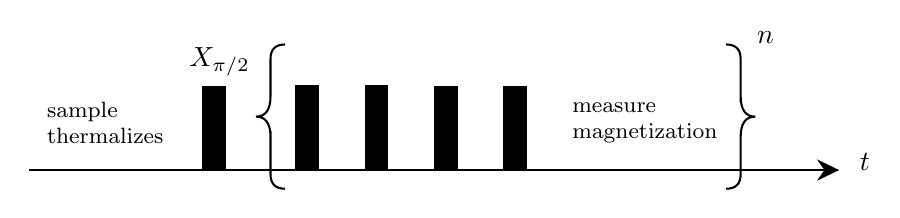
\begin{tikzpicture}[x=0.75pt,y=0.75pt,yscale=-1,xscale=1]
%uncomment if require: \path (0,300); %set diagram left start at 0, and has height of 300

%Straight Lines [id:da3553357763402164] 
\draw    (7,139.5) -- (394.5,139.5) ;
\draw [shift={(397.5,139.5)}, rotate = 180] [fill={rgb, 255:red, 0; green, 0; blue, 0 }  ][line width=0.08]  [draw opacity=0] (10.72,-5.15) -- (0,0) -- (10.72,5.15) -- (7.12,0) -- cycle    ;
%Shape: Rectangle [id:dp9462927331579177] 
\draw  [fill={rgb, 255:red, 0; green, 0; blue, 0 }  ,fill opacity=1 ] (91,99.5) -- (101.5,99.5) -- (101.5,139.5) -- (91,139.5) -- cycle ;
%Shape: Brace [id:dp5361701357698033] 
\draw   (130.5,79) .. controls (125.83,79) and (123.5,81.33) .. (123.5,86) -- (123.5,103.75) .. controls (123.5,110.42) and (121.17,113.75) .. (116.5,113.75) .. controls (121.17,113.75) and (123.5,117.08) .. (123.5,123.75)(123.5,120.75) -- (123.5,141.5) .. controls (123.5,146.17) and (125.83,148.5) .. (130.5,148.5) ;
%Shape: Brace [id:dp6964209405349638] 
\draw   (343,148.5) .. controls (347.67,148.5) and (350,146.17) .. (350,141.5) -- (350,123.75) .. controls (350,117.08) and (352.33,113.75) .. (357,113.75) .. controls (352.33,113.75) and (350,110.42) .. (350,103.75)(350,106.75) -- (350,86) .. controls (350,81.33) and (347.67,79) .. (343,79) ;
%Shape: Rectangle [id:dp10957639024886712] 
\draw  [fill={rgb, 255:red, 0; green, 0; blue, 0 }  ,fill opacity=1 ] (136,99) -- (146.5,99) -- (146.5,139) -- (136,139) -- cycle ;
%Shape: Rectangle [id:dp4589647059466161] 
\draw  [fill={rgb, 255:red, 0; green, 0; blue, 0 }  ,fill opacity=1 ] (169.33,99) -- (179.83,99) -- (179.83,139) -- (169.33,139) -- cycle ;
%Shape: Rectangle [id:dp07946714725560555] 
\draw  [fill={rgb, 255:red, 0; green, 0; blue, 0 }  ,fill opacity=1 ] (202.66,99.5) -- (213.16,99.5) -- (213.16,139.5) -- (202.66,139.5) -- cycle ;
%Shape: Rectangle [id:dp016286675726323585] 
\draw  [fill={rgb, 255:red, 0; green, 0; blue, 0 }  ,fill opacity=1 ] (236,99.5) -- (246.5,99.5) -- (246.5,139.5) -- (236,139.5) -- cycle ;

% Text Node
\draw (406,129.9) node [anchor=north west][inner sep=0.75pt]    {$t$};
% Text Node
\draw (98.94,87.19) node    {$X_{\pi /2}$};
% Text Node
\draw (43.87,116.75) node  [font=\footnotesize] [align=left] {sample\\thermalizes};
% Text Node
\draw (356.5,71.4) node [anchor=north west][inner sep=0.75pt]    {$n$};
% Text Node
\draw (303.87,116.75) node  [font=\footnotesize] [align=left] {measure\\magnetization};


\end{tikzpicture}

    \caption{A typical NMR experiment, including initializing the state, a $\pi/2$-pulse to measure magnetization in the xy-plane, and many repetitions of a pulse sequence and magnetization measurements. After each pulse sequence (between the brackets), the dynamics appear to have evolved due to an engineered Hamiltonian.}
    \label{fig:NMR-Pulse-Train}
\end{figure}

% TODO put in diagram(s) showing FID, spectrum
% TODO do this if I have time...
% \begin{figure}[H]
%     \centering
%     \includegraphics[width=.75\textwidth]{example-image}
%     % TODO replace this with my own data
%     \caption{An observed FID from an NMR experiment and the corresponding spectrum.}
%     \label{fig:NMR-FID-spectrum}
% \end{figure}

If the NMR sample is a liquid, then the sample's molecules are constantly tumbling past each other. As a result, dipolar interactions between spins from different molecules are not constant over the course of the experiment, and in aggregate the dipolar interactions are averaged to zero. This is called ``motional averaging'' of the dipolar interactions
\[
H_{\text{int}} \longrightarrow H_\text{CS}
\]
The chemical shifts for each spin do stay constant (because the local magnetic field due to molecular structure stays the same), so the resulting spectrum clearly resolves chemical shift peaks. Recall that $H_Z$ is not present in the rotating frame.

In contrast, motional averaging does not occur in solid-state NMR. Because the spins are in fixed positions relative to other spins in the sample, dipolar interactions affect the net magnetization of the sample and lead to a broadening of the peaks in the spectrum. This line-broadening inhibits accurate measurements of chemical shifts in solid samples. See figure~\ref{fig:NMR-averaging} for a comparison of spectra between liquid- and solid-state NMR.

\begin{figure}[H]
    \centering
    \includegraphics[width=.6\textwidth]{1H-NMR.jpg}
    \caption{NMR spectra for a solid sample, solid sample with magic-angle spinning, and liquid sample. The goal of NMR spectroscopy is to decouple dipolar interactions (top) so that the peaks can be clearly resolved (bottom). Magic angle spinning (MAS) is one technique for narrowing linewidths in solid samples. From \cite{Ottowa-NMR}.}
    \label{fig:NMR-averaging}
\end{figure}



% TODO also talk about simulation, sensing


% \section{Quantum Control}
%
% Quantum control theory encompasses many different problems, but they each involve driving quantum phenomena in a desired way using a set of control parameters. Quantum control problems include transforming an initial state $\rho(0)$ to a final state $\rho(T)$, creating a specified unitary transformation $U(T)$, or engineering interactions between a subsystem and its environment.\cite{Dong_2010}\footnote{In this work, only closed quantum systems are considered, so bath engineering is not considered.} Systems can be controlled by manipulating parameters in the Hamiltonian, such as the strength or orientation of an external magnetic field (as in NMR).
%
% The Hamiltonian in the context of quantum control can be expressed as
% \begin{equation}
%     H(t) = H_{\text{sys}} + H_{\text{ctrl}}(t)
% \end{equation}
% where $H_{\text{sys}}$ includes interactions in the system that we cannot control, and $H_{\text{ctrl}}(t)$ includes all interactions that we \emph{can} control. In many situations the control Hamiltonian can be expressed as
% \[
% H_{\text{ctrl}}(t) = \sum_k u_k(t) H_k
% \]
% where $\{H_k\}$ is a set of time-independent Hermitian operators and $\{u_k(t)\}$ are real-valued control parameters. In equation~\ref{eq:nmr-ham}, $H_{\text{int}} = H_{\text{sys}}$  and $H_{\text{rf}}(t) = H_{\text{ctrl}}(t)$.



\section{Hamiltonian Engineering}

% Closely related to creating a desired unitary transformation $U(T)$,
Hamiltonian engineering is an important problem within the broader field of quantum control. The goal of Hamiltonian engineering is to choose control parameters $\{u_k(t)\}$ so that, when measured stroboscopically\footnote{Stroboscopically means measured at regular intervals $0, T, 2T, \dots$.}, the system appears to evolve under a target effective Hamiltonian $H_{\text{eff}}$ instead of the system Hamiltonian $H_{\text{sys}}$. In most cases the target Hamiltonian is time-independent.

If we are able to engineer an effective Hamiltonian, then we have also created a unitary transformation $U(T) = \exp{-i H_{\text{eff}} T}$. Conversely, if we have implemented a unitary transformation $U(T)$, then there exists an effective time-independent Hamiltonian that characterizes the dynamics over time $T$ (note that this Hamiltonian is not unique).

\subsection{Average Hamiltonian Theory}\label{sec:AHT}

Average Hamiltonian theory (AHT) provides a framework with which the Hamiltonian engineering problem can be approached. The following presentation of AHT is inspired by \cite{brinkmann_2016, gerstein-dybowski, 1976ii}.

For a particular Hamiltonian $H(t)$, the propagator $U(t)$ is defined by equation~\ref{eq:propagator-de}
\[
i \ddt{U(t)} = H(t) U(t), U(0) = \identity
\]
As the name suggests, average Hamiltonian theory lets us express the propagator $U(t)$ at each time $t$ in terms of an \emph{average} time-independent Hamiltonian $\overline{H}$
\[
U(t) = \exp\left\{-i \overline{H}(t) t \right\}
\]
The above equation seems to suggest that $\overline{H}(t)$ is not time-independent--it is explicitly dependent on time! It is true that $\overline{H}(t)$ itself is not time-independent, but \emph{given} a time $T$, we can find $\overline{H}(T)$ so that the propagator $U(T)$ can be expressed \emph{as though} the Hamiltonian were $\overline{H}(T)$ for the time interval $t \in [0, T]$.

How then do we determine the average Hamiltonian? One approach is to use the Magnus Expansion \cite{Blanes_2009,2010EJPh...31..907B}. Given the propagator differential equation (equation~\ref{eq:propagator-de}), the Magnus Expansion begins with the ansatz that an exponential solution exists
\[
U(t) = \exp\{\Omega(t)\}, \Omega(0) = 0
\]
and proceeds by finding a series expansion for $\Omega(t)$
\[
\Omega(t) = \sum_k \Omega_k(t)
\]
The first few terms are presented below
\begin{align*}
    \Omega_1(t) &= -i \int_0^t dt_1 H(t_1) \\
    \Omega_2(t) &= -\frac{1}{2} \int_0^t dt_1 \int_0^{t_1} dt_2 [H(t_1), H(t_2)] \\
    \vdots
\end{align*}
Derivations of the Magnus Expansion can be found in
\cite{gerstein-dybowski,Blanes_2009,2010EJPh...31..907B}.

From $\Omega(t)$, an expression for the average Hamiltonian can be derived by making the comparison
\[
\Omega(t) = -i \overline{H}(t) t \implies \overline{H}(t) = \frac{i}{t} \Omega(t)
\]
This then gives us a series expansion for the average Hamiltonian $\overline{H}(t) = \sum_k \overline{H}^{(k)}(t)$, with the first few terms given below.
\begin{align}
    \label{eq:AHT-term-0}
    \overline{H}^{(0)} &= \frac{1}{t} \int_0^{t} dt_1 H(t_1) \\
    \label{eq:AHT-term-1}
    \overline{H}^{(1)} &= \frac{1}{2it} \int_0^{t} dt_1 \int_0^{t_1} dt_2
        \left[H(t_1), H(t_2)\right] \\
    \label{eq:AHT-term-2}
    \overline{H}^{(2)} &= -\frac{1}{6t}
    \int_0^{t} dt_1 \int_0^{t_1} dt_2 \int_0^{t_2} dt_3
    \left\{
    \left[H(t_1), \left[H(t_2), H(t_3)\right]\right] \right. \\
    & \hspace{12em} + \left.
    \left[\left[H(t_1), H(t_2)\right], H(t_3)\right]
    \right\}
\end{align}
Although there appears to be a simple pattern to the terms, this is not the case. Higher-order terms can be determined through a recursive relationship or through particularly complicated explicit forms.

The Magnus Expansion converges when
\begin{equation}\label{eq:AHT-convergence}
    \int_0^t dt_1 ||H(t)||_2 \ll 1
\end{equation}
which effectively requires that we consider timescales much smaller than the natural timescale of the Hamiltonian.\footnote{A much more detailed overview regarding convergence can be found in \cite{Blanes_2009}.} This is also written more succinctly as $||H||t \ll 1$.

Because convergence requires the norm of the Hamiltonian to be small, there are cases when working in the interaction frame of a strong interaction is desirable. In NMR, going from the rotating frame (of the Zeeman interaction) to the interaction frame of the rf field removes the strong $H_\text{rf}$ term from the nuclear spin Hamiltonian. This interaction frame is commonly called the ``toggling frame.''
\[
H(t) = H_{\text{int}} + H_{\text{rf}}(t) \implies \widetilde{H}(t) = \widetilde{H}_{\text{int}}(t)
\]
In the toggling frame, the Magnus Expansion can again be used to determine the average Hamiltonian $\overline{\widetilde{H}}(t)$, but using $\widetilde{H}_{\text{int}}(t)$ in place of $H(t)$ in equation~\ref{eq:AHT-term-0}. The upshot is that by going into the toggling frame, the smaller-norm average Hamiltonian converges for longer time values.

At this point, the identification of an ``average Hamiltonian'' is of little benefit: $\overline{H}(t)$ might be different at different times, and it may be the average Hamiltonian in the \emph{toggling} frame instead of the lab frame. To address these concerns, we can require that $H_\text{rf}(t)$ be ``cyclic'' and ``periodic.'' For a fixed time $T>0$,
\begin{align}\label{eq:AHT-constraints}
    U_{\text{rf}}(T) &= \identity & \quad \text{(cyclic)} \\
    H_{\text{rf}}(t + NT) &= H_{\text{rf}}(t), N \in \Z & \quad \text{(periodic)}
\end{align}
$T$ is called the ``cycle time'' and should be short enough so that the Magnus Expansion converges.
The cyclic and periodic properties ensure that the average Hamiltonian is \emph{the same} and that the toggling frame coincides with the rotating frame at multiples of the cycle time $NT$.
% TODO ^ is confusing...

The AHT framework permits continuous control via the rf field, but we will focus on discrete control, where a finite set of rf field pulses can be applied at multiples of time $\tau$. The set of pulses we will consider are $\pi/2$-pulses about the x- or y-axis, which we will label as $\{ X, Y, \overline{X}, \overline{Y} \}$ where the bar denotes a $-\pi/2$ rotation. An $X$ pulse corresponds to the unitary operator
\begin{equation}\label{eq:X-pulse}
    U_X = \exp\left\{-i
        \left[
            \pi/2 \left(\sum_j I_x^{(j)}\right) + H_{\text{int}} t_p
        \right]
    \right\}
\end{equation}
where $t_p$ is the pulse duration. Pulses along the $y$-axis swap the $I_x$ operator with $I_y$, and reverse rotations negate the $\pi/2$ term. In the delta-pulse limit (i.e. $t_p = 0$), an $X$ pulse corresponds to the unitary operator $U_X = \exp\{-i \pi/2 \sum_j I_x^{(j)}\}$ and a $Y$ pulse similarly corresponds to $U_Y = \exp\{-i \pi/2 \sum_j I_y^{(j)}\}$.
% note that I_x is the spin operator, so I_x = hbar/2 * sigma_x

\subsection{WAHUHA-4 Pulse Sequence}\label{subsec:WHH-4}

One of the first pulse sequences developed for Hamiltonian engineering in NMR was the WAHUHA-4 pulse sequence (WHH-4).\cite{PhysRevLett.20.180} The pulse sequence is defined as
\begin{equation}
    \tau, X, \tau, \overline{Y}, \tau, \tau, Y, \tau, \overline{X}, \tau
\end{equation}
where the sequence should be read from left to right (an $X$ pulse is applied first). The pulse sequence is also shown in figure~\ref{fig:WHH-4}.

\begin{figure}[H]
    \centering
    

\tikzset{every picture/.style={line width=0.75pt}} %set default line width to 0.75pt        

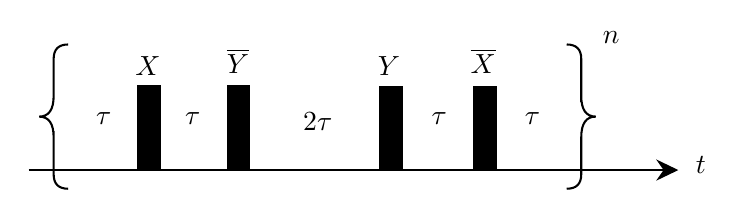
\begin{tikzpicture}[x=0.75pt,y=0.75pt,yscale=-1,xscale=1]
%uncomment if require: \path (0,300); %set diagram left start at 0, and has height of 300

%Straight Lines [id:da6050772876669203] 
\draw    (113.5,159.5) -- (423.5,159.5) ;
\draw [shift={(426.5,159.5)}, rotate = 180] [fill={rgb, 255:red, 0; green, 0; blue, 0 }  ][line width=0.08]  [draw opacity=0] (10.72,-5.15) -- (0,0) -- (10.72,5.15) -- (7.12,0) -- cycle    ;
%Shape: Rectangle [id:dp03677959381184914] 
\draw  [fill={rgb, 255:red, 0; green, 0; blue, 0 }  ,fill opacity=1 ] (166,119) -- (176.5,119) -- (176.5,159) -- (166,159) -- cycle ;
%Shape: Rectangle [id:dp9515559699003447] 
\draw  [fill={rgb, 255:red, 0; green, 0; blue, 0 }  ,fill opacity=1 ] (209.33,119) -- (219.83,119) -- (219.83,159) -- (209.33,159) -- cycle ;
%Shape: Rectangle [id:dp3750218499878627] 
\draw  [fill={rgb, 255:red, 0; green, 0; blue, 0 }  ,fill opacity=1 ] (282.66,119.5) -- (293.16,119.5) -- (293.16,159.5) -- (282.66,159.5) -- cycle ;
%Shape: Rectangle [id:dp4039169654303607] 
\draw  [fill={rgb, 255:red, 0; green, 0; blue, 0 }  ,fill opacity=1 ] (328,119.5) -- (338.5,119.5) -- (338.5,159.5) -- (328,159.5) -- cycle ;
%Shape: Brace [id:dp43500153185683443] 
\draw   (132.51,99) .. controls (127.84,99) and (125.51,101.33) .. (125.51,106) -- (125.51,123.75) .. controls (125.51,130.42) and (123.18,133.75) .. (118.51,133.75) .. controls (123.18,133.75) and (125.51,137.08) .. (125.51,143.75)(125.51,140.75) -- (125.51,161.5) .. controls (125.51,166.17) and (127.84,168.5) .. (132.51,168.5) ;
%Shape: Brace [id:dp32462909095886316] 
\draw   (372.71,168.5) .. controls (377.38,168.5) and (379.71,166.17) .. (379.71,161.5) -- (379.71,143.75) .. controls (379.71,137.08) and (382.04,133.75) .. (386.71,133.75) .. controls (382.04,133.75) and (379.71,130.42) .. (379.71,123.75)(379.71,126.75) -- (379.71,106) .. controls (379.71,101.33) and (377.38,99) .. (372.71,99) ;

% Text Node
\draw (433.5,151.4) node [anchor=north west][inner sep=0.75pt]    {$t$};
% Text Node
\draw (170.94,109.19) node    {$X$};
% Text Node
\draw (214.27,107.19) node    {$\overline{Y}$};
% Text Node
\draw (287.1,109.19) node    {$Y$};
% Text Node
\draw (332.44,107.19) node    {$\overline{X}$};
% Text Node
\draw (144.5,130.4) node [anchor=north west][inner sep=0.75pt]    {$\tau $};
% Text Node
\draw (187.38,130.4) node [anchor=north west][inner sep=0.75pt]    {$\tau $};
% Text Node
\draw (244.26,130.4) node [anchor=north west][inner sep=0.75pt]    {$2\tau $};
% Text Node
\draw (306.14,130.4) node [anchor=north west][inner sep=0.75pt]    {$\tau $};
% Text Node
\draw (351,130.4) node [anchor=north west][inner sep=0.75pt]    {$\tau $};
% Text Node
\draw (388.69,91.4) node [anchor=north west][inner sep=0.75pt]    {$n$};


\end{tikzpicture}

    \caption{The WHH-4 sequence repeated $n$ times in a pulse train. If the magnetization of the sample is measured after each WHH-4 sequence, the dynamics will appear to evolve according to the average Hamiltonian given below.}
    \label{fig:WHH-4}
\end{figure}

The propagator for a single cycle of the WHH-4 sequence is
\[
U_{\text{WHH-4}} =
    \exp\{-i H_{\text{int}} \tau\} U_{\overline{X}}
    \exp\{-i H_{\text{int}} \tau\} U_Y
    \exp\{-i H_{\text{int}} 2\tau\} U_{\overline{Y}}
    \exp\{-i H_{\text{int}} \tau\} U_X
    \exp\{-i H_{\text{int}} \tau\}
\]

Now, using AHT, we express $U_{\text{WHH-4}} = \exp\{-i \overline{H}_{\text{WHH-4}} 6\tau\}$ and find an approximation for the average Hamiltonian $\overline{H}_{\text{WHH-4}}$. The toggling frame propagator as well as the toggled $I_z^{(j)}$ and $I_z^{(j)}I_z^{(k)}$ terms are determined by the four pulses in the sequence. For $t \in [0, \tau]$, the toggling frame corresponds to the lab frame.
But after the $X$ pulse, the toggling frame propagator is now $U_X$, so the toggled spin terms are $\widetilde{I_z}^{(j)} = U_X^\dagger I_z^{(j)} U_X = I_y^{(j)}$
\footnote{
This can be seen by noting that $\exp\{-i \theta I_x\} = \exp\{-i \theta/2 \sigma_x\} = \cos(\theta/2) \identity - i\sin(\theta/2) \sigma_x$, then using the commutation relations for Pauli matrices to simplify. As a rule of thumb, $U_X$ rotates the lab frame's y-axis into the z-axis so that $\widetilde{I}_z = I_y$, and $U_Y$ rotates z into y.
}
The toggling frame and corresponding terms for each time interval are given in table~\ref{tab:WHH-4}.

\begin{table}[H]
    \centering
    \caption{The WHH-4 toggling frame propagator and toggled terms at different time intervals.}
    \label{tab:WHH-4}
    \begin{tabular}{c c c c}
        Time interval & Toggling frame propagator $U_{\text{rf}}$ & $\widetilde{I_z}$ & $\widetilde{I_z}^{(j)}\widetilde{I_z}^{(k)}$ \\
        \hline
        $[0, \tau]$ & $\identity$ & $I_z$ & $I_z^{(j)}I_z^{(k)}$ \\
        $[\tau, 2\tau]$ & $U_X$ & $I_y$ & $I_y^{(j)}I_y^{(k)}$ \\
        $[2\tau, 4\tau]$ & $U_{\overline{Y}} U_X$ & $I_x$ & $I_x^{(j)}I_x^{(k)}$ \\
        $[4\tau, 5\tau]$ & $U_X$ & $I_y$ & $I_y^{(j)}I_y^{(k)}$ \\
        $[5\tau, 6\tau]$ & $\identity$ & $I_z$ & $I_z^{(j)}I_z^{(k)}$ \\
    \end{tabular}
\end{table}

Note that in the dipolar interaction $H_D$, the isotropic term $\mathbf{I}^{(j)} \cdot \mathbf{I}^{(k)}$ is invariant under rotations and therefore not transformed by the toggling frame.

We see that WHH-4 is cyclic because $U_{\text{rf}}(6\tau) = \identity$, and the applying the WHH-4 sequence repeatedly would satisfy the periodic requirement. To determine the lowest-order term in the Magnus Expansion $\overline{H}^{(0)}$, we use the toggled terms from table~\ref{tab:WHH-4} in equation~\ref{eq:AHT-term-0}.
\begin{align*}
    \overline{H}^{(0)} &= \frac{1}{6\tau} \int_0^{6\tau} dt_1
    \widetilde{H}_{\text{int}}(t_1) \\
    &= \frac{1}{6\tau} \left[
        \sum_j \delta_j \left(2\tau I_z^{(j)} + 2\tau I_y^{(j)} + 2\tau I_x^{(j)} \right) +
        \sum_{jk} d_{jk} \left(3(
            2\tau I_z^{(j)}I_z^{(k)} + 2\tau I_y^{(j)}I_y^{(k)} + 2\tau I_x^{(j)}I_x^{(k)}
        ) - 6\tau \mathbf{I^{(j)}} \cdot \mathbf{I^{(k)}} \right)
    \right] \\
    &= \left[
        1/3 \sum_j \delta_j \left(I_z^{(j)} + I_y^{(j)} + I_x^{(j)} \right) +
        \sum_{jk} d_{jk} \left(I_z^{(j)}I_z^{(k)} + I_y^{(j)}I_y^{(k)} + I_x^{(j)}I_x^{(k)} - \mathbf{I}^{(j)} \cdot \mathbf{I}^{(k)} \right)
    \right] \\
    &= 1/3 \sum_j \delta_j \left(I_z^{(j)} + I_y^{(j)} + I_x^{(j)} \right)
\end{align*}
The WHH-4 sequence, to lowest order, refocuses or ``cancels out'' the dipolar interaction between spins while retaining the chemical shift term. Instead of the principal axis being along z, however, the spin operator acts along the diagonal axis $(1,1,1)$.

\subsection{CORY-48 Pulse Sequence}\label{subsec:CORY48}

AHT can be taken even further than the WHH-4 sequence by considering higher-order terms in the Magnus Expansion. The CORY48 sequence is a 72$\tau$, 48-pulse sequence that was designed to decouple all interactions so that $H_{\text{eff}} = 0$ \cite{CORY1990205}. Furthermore, the CORY48 sequence decouples the dipolar interactions to \emph{second order}, and is robust to errors including pulse rotation errors and resonance offset errors. The full sequence is presented in equation~\ref{eq:CORY48}.

\begin{equation}\label{eq:CORY48}
\begin{aligned}
    X, \tau, Y, 2\tau, \overline{X}, \tau, Y, 2\tau, X, \tau, Y, 2\tau,
    X, \tau, Y, 2\tau, X, \tau, \overline{Y}, 2\tau, X, \tau, Y, 2\tau \\
    %
    \overline{Y}, \tau, \overline{X}, 2\tau, Y, \tau, \overline{X}, 2\tau,
    \overline{Y}, \tau, \overline{X}, 2\tau, \overline{Y}, \tau, \overline{X},
    2\tau, \overline{Y}, \tau, X, 2\tau, \overline{Y}, \tau, \overline{X},
    2\tau \\
    %
    \overline{X}, \tau, Y, 2\tau, \overline{X}, \tau, \overline{Y}, 2\tau,
    \overline{X}, \tau, Y, 2\tau, X, \tau, \overline{Y}, 2\tau, \overline{X},
    \tau, \overline{Y}, 2\tau, X, \tau, \overline{Y}, 2\tau \\
    %
    Y, \tau, \overline{X}, 2\tau, Y, \tau, X, 2\tau, Y, \tau, \overline{X}, 2\tau, \overline{Y}, \tau, X, 2\tau, Y, \tau, X, 2\tau, \overline{Y}, \tau, X, 2\tau
\end{aligned}
\end{equation}


The full AHT analysis is not presented here, but one can imagine evaluating the three lowest-order terms from equations~\ref{eq:AHT-term-0} to~\ref{eq:AHT-term-2} using each of the $48$ time intervals. The lowest-order term is not difficult to calculate, but the higher-order terms quickly become intractable as the integrals include more and more nested commutators.

By comparing the average correlation (explained in greater depth in section~\ref{sec:experimental}) for an FID, the WHH-4 sequence, and the CORY48 sequence in an adamantane, it is clear that the longer CORY48 sequence outperforms the shorter WHH-4 sequence in decoupling interactions and extending the coherence time (see figure~\ref{fig:decay_plot_AHT}).


\begin{figure}[H]
    \centering
    \includegraphics[width=.7\textwidth]{decay_plot.pdf}
    \caption{The average correlation for a free induction decay (FID), the WHH-4 sequence, and the CORY48 sequence in an adamantane sample. Both the WHH-4 and the CORY48 extend the coherence times of the sample, but CORY48 achieves nearly two orders of magnitude greater improvement. The $T_1$ time for adamantane is shown at $t=1$s.}
    \label{fig:decay_plot_AHT}
\end{figure}

However, AHT may not be a suitable framework with which to develop pulse sequences that improve upon CORY48. The computational resources required to decouple interactions to higher orders would be significant.
